\documentclass[a4paper, 10pt, conference]{IEEEtran}

\IEEEoverridecommandlockouts

\usepackage[utf8]{inputenc}
\usepackage[T1]{fontenc}
\usepackage[colorlinks=true,linkcolor=black,anchorcolor=black,citecolor=black,filecolor=black,menucolor=black,runcolor=black,urlcolor=black]{hyperref}
\usepackage{graphicx}
\usepackage[ngerman]{babel}
\usepackage[style=ieee]{biblatex}

\addbibresource{references.bib}

\graphicspath{ {./images/} }

\begin{document}

\makeatletter
\newcommand{\linebreakand}{%
\end{@IEEEauthorhalign}
\hfill\mbox{}\par
\mbox{}\hfill\begin{@IEEEauthorhalign}
}
\makeatother

\title{\LARGE \bf
Konzeptpapier: Battleship
}

\author{

\IEEEauthorblockN{Jakob Götz} 
\IEEEauthorblockA{\textit{j.goetz@oth-aw.de}}\and
\IEEEauthorblockN{Uwe Kölbel} 
\IEEEauthorblockA{\textit{u.koelbel@oth-aw.de}}\and
\IEEEauthorblockN{Maximilian Schlosser} \IEEEauthorblockA{\textit{m.schlosser@oth-aw.de}}\and
\IEEEauthorblockN{Oliver Schmidts} \IEEEauthorblockA{\textit{o.schmidts@oth-aw.de}}\linebreakand
\IEEEauthorblockN{Jan Schuster} 
\IEEEauthorblockA{\textit{j.schuster@oth-aw.de}}\and
\IEEEauthorblockN{Philipp Seufert} 
\IEEEauthorblockA{\textit{p.seufert@oth-aw.de}}\and
\IEEEauthorblockN{Fabian Wagner} 
\IEEEauthorblockA{\textit{f.wagner@oth-aw.de}}
}

\maketitle
\thispagestyle{empty}
\pagestyle{empty}


\begin{abstract}
    Wir beschäftigen uns mit der Speicherung und Suche vernetzter Informationen von Videospielen.
    Dazu stellen wir \textit{SGDb} vor -- eine webbasierte Anwendung mit einer Graphen-basierten Suche von Videospielen.
\end{abstract}


\section{Einleitung}\label{sec:einleitung}

Das erste Videospiel \textit{Tennis for Two} aus dem Jahr 1958 ebnete den Weg für die Spieleindustrie. Über Jahrzehnten hinaus kamen immer mehr verschiedene Spiele auf den Markt, die sich in ihrer Art und Weise unterscheiden. Mit den heutigen Videospielen ist es möglich, sich mit Spielern aus der ganzen Welt zu messen oder gemeinsam zu spielen. Aus den unzählig veröffentlichen Videospielen ist eine breite Palette an Genres entstanden. Dabei wird in der Spieleindustrie grob in sechs Kategorien unterschieden, hierbei zählen die Strategie- und Action-Spiele zu den beliebtesten Genres~\cite{statistica}. Zu den anderen vier Kategorien zählen die Rollen-, Abenteuer-, Simulationen- und sonstige Spiele. Jedes dieser Kategorien besitzt weitere Unterkategorien, die sich in ihrer Art und Weise unterscheiden.\\

Um einen Überblick zu erhalten, wie die Spiele zusammenhängen, präsentieren wir hier eine plattformunabhängige Anwendung, welche die Spiele in einem Graphen darstellt. In Abschnitt~\ref{sec:verwandte_arbeiten} des Konzeptpapiers werden bereits bestehende Anwendungen vorgestellt, die sich mit der Kategorisierung von Spielen und Darstellung von Graphen beschäftigen.
In Abschnitt~\ref{sec:anforderungen} werden die Anforderungen in Form von User Stories beschrieben. Zum Schluss wird auf die geplanten Technologien bei der Umsetzung des Projekts eingegangen, welche in Abschnitt~\ref{sec:methoden} beschrieben werden.


\section{Verwandte Arbeiten}\label{sec:verwandte_arbeiten}

Die \textit{Internet Video Games Database} (IGDB)~\cite{igdb} gibt einen Eindruck, was ein Nutzer von einer Videospieldatenbank erwarten kann. IGDB umfasst derzeit 217.233 Spiele, eine Suchfunktion, die Möglichkeit Videospiele zu entdecken (z.B.\ kürzlich veröffentlichte Videospiele), und eine Entwickler-API. Über die API können Entwickler auf die Videospieldaten mittels Protokolle wie REST oder ProtoBuf zugreifen.

Wie die Visualisierung eines Graphen möglicherweise aussehen kann, demonstriert die Anwendung Obsidian. Diese erstellt aus von Nutzern kreierten Markdown Dateien eine Graphenoberfläche. Über Verlinkungen zwischen den Markdown Dateien wächst der Graph an. Der Nutzer kann den Graph filtern oder gewisse Teile daraus hervorheben (vgl. Abbildung~\ref{fig:obsidian}).

\begin{figure}[thpb]
    \centering
    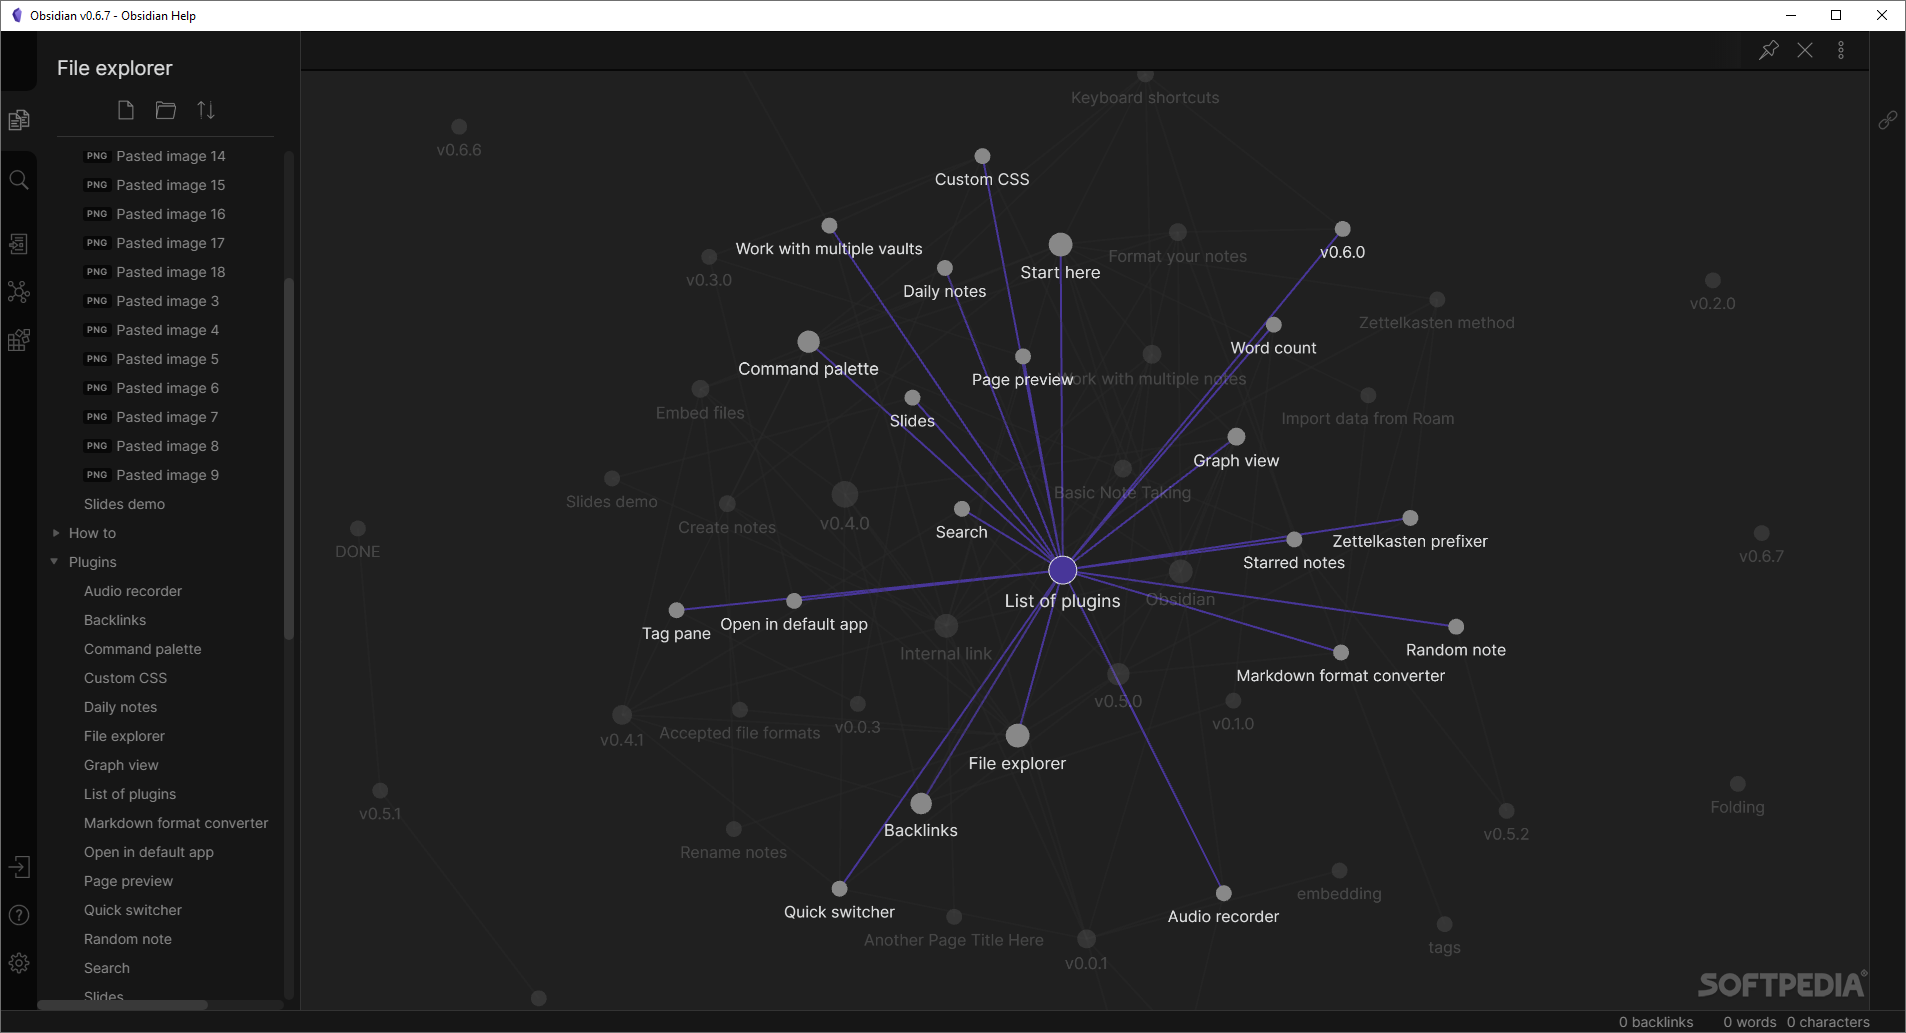
\includegraphics[scale=0.17]{obsidian}
    \caption{Obsidian Benutzeroberfläche~\cite{obsidian}}
    \label{fig:obsidian}
\end{figure}


\section{Anforderungen}\label{sec:anforderungen}

In der Anforderungsanalyse wurden drei primäre Komponenten identifiziert, die es umzusetzen gilt: (1) Die Menüführung (2) das Gameplay und (3) das Dashboard.


\subsection{Menüführung}
Als Benutzer möchte ich ein intuitiv zu bedienendes Menü, in dem ich:
\begin{itemize}
	\item meinen Benutzernamen eingeben kann,
	\item ein Spiel starten kann,
	\item eine Anleitung aufrufen kann und
	\item meinen Benutzernamen eingeben kann,
	\item ein Dashboard mit Statistiken aufrufen kann.
\end{itemize}

Als Benutzer möchte ich zwischen verschiedenen Spielmodi wählen können:
\begin{itemize}
	\item Gegen Computer
	\item Gegen zufälligen Gegner
	\item Gegen Freund
\end{itemize}

\subsection{Gameplay}
Im Spiel möchte ich nach folgenden Regeln spielen:
\begin{itemize}
	\item Zu Beginn muss jeder Spieler eine festgelegte Anzahl an Schiffen unterschiedlicher Größe platzieren.
	\item Die Spieler dürfen abwechselnd einen Schuss abfeuern.
	\item Sind alle Schiffe eines Spielers versenkt, hat dieser Spieler verloren.
\end{itemize}

Im Spiel möchte ich:
\begin{itemize}
	\item meine Schiffe zufällig oder händisch auf dem Spielfeld platzieren können
	\item mit den Waffen meiner Schiffe feuern können
	\item meine Treffer und die verfehlten Schüsse auf dem Spielfeld erkennen können
	\item ein übersichtliches Spielfeld mit allen relevanten Informationen 
	\item (optional) mit meinem Gegner kommunizieren können
	\item (optional) Spiel pausieren, später fortsetzen
\end{itemize}

\subsection{Leaderboard / Dashboard}
Als Benutzer möchte ich ein Dashboard, das Informationen über vergangene Spiele darstellt. Denkbar sind:
\begin{itemize}
	\item Eine Bestenliste
	\item Anzahl der benötigten Schüsse bis zum Sieg
	\item Beliebteste Schiffspositionen
	\item Gewinnrate gegen Computer
\end{itemize}


\section{Methoden}\label{sec:methoden}

Ziel bei der Entwicklung und bei der späteren Verwendung ist eine plattformunabhängige Anwendung, die eine Schnittstelle für die \textit{Linked Open Data Cloud} als auch der Bedienoberfläche der Anwendung bereitstellt. Daraus ergeben sich folgende technische Schlüsselbausteine:

Für die Repräsentation der semantischen Daten im Frontend wird das Framework Svelte verwendet. Die Daten werden voraussichtlich in einer Ontotext GraphDB Instanz persistiert. Im Backend wird FastAPI für eine REST-Schnittstelle und RDFLib zum arbeiten mit RDF verwendet. Die Kommunikation zwischen Frontend und Backend wird über die RESTful-API abgewickelt. Die einzelnen Komponenten der Anwendung (Frontend, Backend und Datenbank) werden mittels Docker \textit{containerisiert}.


\printbibliography

\end{document}
